\section{词法}
codger源程序由一系列具有独立意义的基本语法单位--单词组成,单词是最小的词法单位,它们不能分割。单词分为8类:关键字,运算符,特殊符号,整数,长整数,浮点数,字符串,标识符,空白符,注释,其中空白符与注释属于无用单词,当被扫描器识别到时,会立刻被弃。

解析器中的语法识别模块用于对codger源程序进行词法分析,从输入字符流中扫描出由字符序列组成的单词。并把识别出的单词交给后面的语法分析模块进一步处理,并在识别过程中检测是否存在非法的单词。
\subsection{关键字}
codger中关键字具有专门的意义与用途,它们不能被当作一般的标识符来使用,这些关键字有:
\begin{quote}
\begin{verbatim}
and, as, attr, break, catch, class, continue, export,
do, elif, else, end, false, finally, for, from, func, 
if, import, in, inherit, new, not, or, print, private, 
protected, public, return, static, then, to, true,
try, while。
\end{verbatim}
\end{quote}
\subsection{标识符}
标识符用于定义变量,函数,类,方法等所使用的名称,解析器没有限定标识符的长度,但在定义标识符时,需要遵守一定的规则:以字母或者下画线开头,后面可以接零个或多个字母、数字、下画线,并且区会字母的大写与小写。用文法表示为:
\begin{quote}
\begin{verbatim}
identifier =(letter|"_"|)(letter|digit|"_")*
digit ="0".."9"
letter =lowercase|uppercase
lowercase ="a".."z"
uppercase ="A".."Z"
\end{verbatim}
\end{quote}
\subsection{特殊符号与运算符}
在codger中,运算符用于指定一种运算方式,特殊符号用于分隔不同的语句或者用于指定某些特定意义的用途。它们有:
\begin{quote}
\begin{verbatim}
 (   )   [   ]   .   ,  +   -   ~   *  ;
 /   %  <<   >>   <   >   <=   >=  ==
 !=   &   ^   | =   +=   -=   *=   /= 
 %=   &=   ^=   |=   >>=   <<=  换行符
\end{verbatim}
\end{quote}
\subsection{整数}
整数是一种与机器平台相关的数据类型,在32位机上,其表示范围为 $-2^{31}$ 到 $2^{31}-1$。而在64位机上,其表示范围为$-2^{63}$ 到 $2^{63}-1$ 。整数的表示范围有限,在设计程序时需要考虑运算结果溢出的情况。整数可以在codger源程序中显示的定义,整数又被分为二进制整数,八进制整数,十进制整数,十六进制整数。二进制整数以0b或者0B开头,后面紧接着一个或多个0或1;八进制整数以0或者0o、0O开头,后面紧接数字一个或多个0-7;十进制整数以1-9开头,后面紧接数字零个或多个0-9,或者是十进制整数只有一位0;十六进制整数以0x或都0X开头,后面紧接一个或者多个数字0-9、a-f、A-F。用文法表示为:
\begin{quote}
\begin{verbatim}
integer =decimalinteger|octinteger|hexinteger|bininteger
decimalinteger = nonzerodigit digit* | "0"
octinteger = "0" ("o" | "O") octdigit+ | "0" octdigit+
hexinteger = "0" ("x" | "X") hexdigit+
bininteger = "0" ("b" | "B") bindigit+
nonzerodigit = "1"..."9"
octdigit = "0"..."7"
bindigit = "0" | "1"
hexdigit:= digit | "a"..."f" | "A"..."F"
\end{verbatim}
\end{quote}

\subsection{长整数}
整数表示范围有限,在进行大数据运算时受到限制,Codger 提贡长整数用于解决这种问题。长整数是一种与机器无关的数据类型,可以进行任意大小的数据运算,不用去考虑数据溢出问题,但是前提是你的计算机有中够大的内存空间,来保存这些数据。 长整数可以在源程序中显示的定义,定义方法同整数一样,只有在后面多了一位字符L或者是l。用文法表示为:
\begin{quote}
 \begin{verbatim}
  longinteger = integer ("l" | "L")
 \end{verbatim}
\end{quote}

\subsection{浮点数}
在codger中采用的是32位浮点数,其数值范围约为:$-3.4*10^{-38}$ 到 $-3.4*10^{38}$ 。浮点数由三个部分组成:整数部分,浮点部分,指数部分。浮点数可以在源程序中显示定义,定义时整数部分与指数部分可以省去。用文法表示浮点数为:
\begin{quote}
 \begin{verbatim}
floatnumber = pointfloat | exponentfloat
pointfloat = [intpart] "." digit+
exponentfloat = (intpart | pointfloat) exponent
intpart = digit+
exponent = ("e" | "E") ["+" | "-"] digit+
 \end{verbatim}
\end{quote}
\subsection{字符串}
字符串可以在源程序中显示定义,使用规则为:以双引号开头和双引号结尾,中间可以是除 \verb \ 和换行符以处的任意字符,其中\verb \ 用于转义其它特殊字符,如果想要以多行的形式书写字符串,需要在每一行的未尾加上\verb \ 。用文法表示为:
\begin{quote}
 \begin{verbatim}
string =`"'stringitem*`"'
stringitem = <any source character except "\" 
				or newline or the quote> |"\"esc_item
esc_item =<any source character >
 \end{verbatim}
\end{quote}
\subsection{注释}
在Codger注释以\#号开头,直到这一行结果,解析器解析源程序,注释中的所有内容都分被忽略掉。用bnf文法表示为:
\begin{quote}
 \begin{verbatim}
comment ="#" cm_item* newline
cm_item =<any source character except newline>
 \end{verbatim}
\end{quote}
\subsection{空白符}
Codger中的空白符由一个或都多个空格或者是制表符组成,程序中的空白符用于区分开不同的单词,或者使源程序的可读性更强。当解析器识别到空白符时,不会对它做任何的处理,只是简单的将它抛弃。用文法表示为:
\begin{quote}
 \begin{verbatim}
white_space =ws_item+
ws_item = space | tab 
 \end{verbatim}
\end{quote}


\newpage
\section{词法识别算法}
在前面一部分给出了在codger中所有的单词,以及描述单词结构的bnf文法,这些文法都是正则文法。正则文法与有限状态机具有等价性,它们之间可以相互转换\footnote{等价性的证明以及转换的方法可以参考``形式语言与自动机理论''}。而词法识别算法通常是通过构造有限状态机的方法来识别源程序中的不同类型的单词,状态机可以使用类似于lex的词法分析软件自动生成,这种方法处理起来简单,只需要遵守词法分析软件的使用规则即可,或者程序员可以通过手工来构造状态机。手工构造相比词法分析软件相比优点在于:
\begin{enumerate}
 \item 词法分析软件有固定处理框架,不能随意改变,限定了程序的灵活性。手工构造则没有这种限制。
 \item 词法分析软件根据一定算法生成有限状态机,其中有许多重复的或者是多余的状态都可以被优化掉。
\end{enumerate}
但手工构造如果处理不好,可能会随着正则语言规模的增大,复杂度也跟着增加,最终可以超出人脑可能处理的限度。下面介绍一种在codger词法分析模块中使用的一种算法--状态链。
\subsection{状态链简介}
在codger解析器的早期版本中,采用状态矩阵\footnote{大多数编译原理书本都会介绍状态矩阵算法,这里不对其进行详细说明}的方法来识别源程序中的单词。但由于状态矩阵算法会随着正则文法规模的增大,复杂度也跟着增加,每次当需要变更每个单词的结构时,都需要更改一大堆数据,使解析器的维护的扩展都变得非常困难,而且极容易出错。最后不得不放弃状态矩阵,而寻找新的方法。

状态链识别法是在codger解析器开发过程中总结出的一种非常实用和高效的算法,之所以命名为状态链,因为状态链算法处理的最多的是状态与状态之间的链接。状态链算法优点再于:
\begin{enumerate}
 \item 随着正则文法规模的变大,其复杂度一般情况下不会增加。
 \item 状态链是一种分治算法,它先通过为每一个不同类型的单词构造子状态机,然后再通过合并算法把子状态机合并在一起,合并时,不需要更改子状态机中的数据和状态,只需增加新的状态链接到子状态机中已有的状态。
 \item 状态机中的每个状态只需要处理它所接受输入事件类型,以及在该输入事件类型下的后继状态,而不用去了解状态机的整体结构。当状态机的结构发生变化时,很多状态都可以直接得到重用,使解析器的维护和扩展变得非常容易。
\end{enumerate}
\subsection{状态的结构}
状态链算法中,许多的状态链接在一起构成一个有限状态机,在每个状态中都会保存与该状态相关的基本信息,这些信息有:
\begin{enumerate}
 \item 状态是否为终态,如果是终态,同时也会保存该状态所属单词的类型,单词类型用于后面的语法分析。
 \item 字符映射数组:字符射数组长度为256,codger源程序是由字符序列组成,每当解析器从源程序中读出一个字符时,该字符的值的范围为:0到255,然后字符映射数组获得输入事件类型。
 \item 状态能接受的输入事件类型,以及在该输入类型下所转换到的后继状态。
\end{enumerate}
用程序来描述为(attr表示属性定义):
\begin{quote}
 \begin{verbatim}
class State
    attr finally        #是否为终态
    attr token          #单词的类型
    attr input_map[256] #字符映射数组
    attr targets[]      #后继状态
end
 \end{verbatim}
\end{quote}
例如:假设状态a为不为终态,在字符`0'到`9'下转移到状态b,在`a'到`f'下转移到状态c,在其它状态下,转换到错误状态。为状态a构造状态数据为:
\begin{quote}
 \begin{verbatim}
State a
    finally=false
    token="unkown"
    input_map=[0,0,0,0,0,0,0,0,0,0,0,0,0,0,0,0
               0,0,0,0,0,0,0,0,0,0,0,0,0,0,0,0
               0,0,0,0,0,0,0,0,0,0,0,0,0,0,0,0
               1,1,1,1,1,1,1,1,1,1,0,0,0,0,0,0
               0,0,0,0,0,0,0,0,0,0,0,0,0,0,0,0
               0,0,0,0,0,0,0,0,0,0,0,0,0,0,0,0
               0,2,2,2,2,2,0,0,0,0,0,0,0,0,0,0
               0,0,0,0,0,0,0,0,0,0,0,0,0,0,0,0
                       .........
               0,0,0,0,0,0,0,0,0,0,0,0,0,0,0,0]
    targets=[err,b,c]
end  
 \end{verbatim}
\end{quote}

其中在input\_map中的省略号为112个0,状态a总共能接受三种输入事件类型,由于数组脚标从零开始,所以三种输入事件类型分别称为输入事件0,输入事件1,输入事件2
\begin{enumerate}
 \item 输人字符`0'到`9'会被映射为第1种输入事件类型,状态a在该输入类型下会转移到后继状态b,状态b保存在targets中的脚标为1的位置
 \item 输入字符`a'到`f'会被映射为第2种输入事件类型,状态a在该输入类型下会转移到后继状态c,状态c保存在targets中的脚标为2的位置
 \item 除`0'到`9'和`a'到`f'以外的所有字符会被映射到第0种输入事件类型,状态a在该输类型下会转移到后断状态err,状态err保存在targets中的脚标为0的位置。状态err是一个内置状态,用于表示源程于中单词存在错误。
\end{enumerate}

input\_map是一个256位的数组,数组元素类型为unsigned char, unsigned char占用一个字节,即一个input\_map需要256字节。但并不是每个状态都需要独自拥有一个字符映射数组。在很多情况下,许多状态的输入事件类型相似,或者是完全相同,它们可以建立一个公有的字符映射数组,用于共享,以提高内存的利用率。例如状态a在符号`c'到`z'转换到状态c,状态b在字符`a'到`f'能转换到状态c,虽然状态a与状态b能接受的输入事件类型不同,但是可能通过合并状态a与状态b输入事件,让它们共享一个字符映射数组。合并方法为:提取出字符`c'到z'与字符`a'到`f'两个序列范围的交集部分为:字符`c'到`f',即现在的有四种输入类型
\begin{quote}
1) 类型0, 字符`a'到`b' \\
2) 类型1, 字符`c'到`f' \\
3) 类型2, 字符`g'到`z' \\
4) 类型3, 除前面字符以外的所有字符。 
\end{quote}
以前状态a是在字符`c'到`z'转换到状态c,现在改为在字符`a'到`b'与字符`c' 到 `f'的情况下转换到c;以前状态b是在字符`c'到`z'转换到状态c,现在改为在字符`c'到`f'与字符`g'到`z'的情况下转移到状态c。在合并字符映射数组后,a的后继状态数组改为[c,c,err,err],b的后继状态数组为[err,c,c,err]。

Codger解析器的词法识别模块大约有90多个状态和10字符映射组成,基本上每种单词类型的所有状态共享一个状态映射数组。词法识别模块所占用的内存大约在4k左右。
\subsection{识别算法}
Codger的词法识别算法是基于有限状态机,在词法识别模块保存了一个完整的,能识别到codger语言中所有单词的有限状态机。当解析器解析codger源程序时,采用最大识别的方法,下面为识别一个单词大概步骤:
\begin{enumerate}
 \item 置当前状态置为有限状态机的开始状态
 \item 从输入字符流中读出一个字符
 \item 根据当前状态与输入字符确定下一个状态,并置当前状态为下一状态
 \item 处理当前状态,当前状态的类型有三种情况:普通状态,终态,错误状态
 \begin{enumerate}
 	\item 普通状态:跳转的步聚2
 	\item 终态:则记录下该状态与输入字符流的位置。并且跳转到步聚2
 	\item 错误状态:查看以前是否到达过终态,如果是则选择最近一次到达的终态,把多识别的字符返回给输入字符流,返回该单词的类型。如果没有到达过终态,则表明源程序中存在词法错误,返回出错信息。
 \end{enumerate}
\end{enumerate}
用代码来描述为:
\begin{quote}
\begin{verbatim}
GetToken(f)                    
    cur_state=begin_state      #设置当前状态为开始状态
    finally_state=Nil          #以及初始化程序数据
    file_pos=Nil
    while true 
        c=f.getchar()                 #从文件读出一个字符
        cur_state=cur_state.next(c)   #获取下一状态
        if cur_state==err         
            if finally_state!= Nil    #以前到达过终态
                f.set_read_pos(file_pos)  
                return finally_state.token  
            else                      #以前没有到达过终态
                return  ERR_TOKEN  
            end
        elif cur_state.finally        #如果为终态
            finally_state=cur_state   #保存该状态
            file_pos=f.get_read_pos   #保存文件的读位置
        end
    end
end 
\end{verbatim}
\begin{center}
 代码4.3.1
\end{center}
其中State.next的代码如下:
\end{quote}
\begin{quote}
\begin{verbatim}
State.next(c)
    input_type=State.input_map[c]    #获取输入类型
    return State.targets[input_type] #找到后继状态并返回
end 
\end{verbatim}
\end{quote}

涉及到识别到错误状态时,读位置的回退操作,回退的平均位移为2,所以代码4.3.1的时间算杂度与基本上与源文件的字符长度成正比。
  
\subsection{状态机的合并}
在前面介绍过,状态链算法是一种分治的算法,其主要思想为先为每个不同类型的单词构造子状态机,然后通过合并算法把子状态机合并成为一个大的综合性的状态机。假设现在有两个状态机:
\begin{quote}
1) 状态机A用于识别正则式[0-7]+abf所表示的语言,如图:figure~\ref{fig:state_a}\\
2) 状态机B用于识别正则式[4-9]+acd所表示的语言,如图:figure~\ref{fig:state_b}
\end{quote}
\begin{figure}
 \centering
 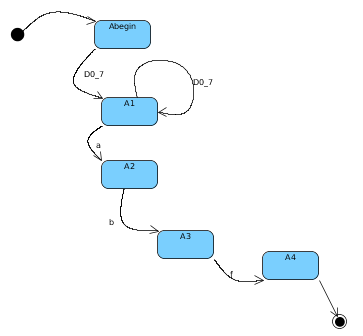
\includegraphics[scale=1]{s_a.png}
 \caption{状态机A}
 \label{fig:state_a}
\end{figure}
为了减少字符映射数组的使用,让状态机A的所有状态共享一个状态映射数组,这样一来,对于每个状态来说就有5种输入类型,同样也就有5个后继状态:
\begin{quote}
1) 数字0到7,命名为 D0\_7  \\
2) 字符a,命名为 S\_a  \\
3) 字符b,命名为 S\_b \\
4) 字符f,命名为 S\_f \\
5) 除以上字符以外的所有字符,命名为 Other
\end{quote}
例如状态机A中的状态A1的后继状态为:[A1,A2,err,err,err] 

同样对状态机B中的所有状态也让它们共享一个状态映射数组,则对于每个状态来说,输入类型有5种,5个后继状态:
\begin{quote}
1) 数字4到9,命名为 D4\_9 \\
2) 字符a,命名为 S\_a \\
3) 字符c,命名为 S\_c \\
4) 字符d, 命名为 S\_d \\
5) 除以上字符以外的所有字符,命名为 Other
\end{quote}
\begin{figure}
 \centering
 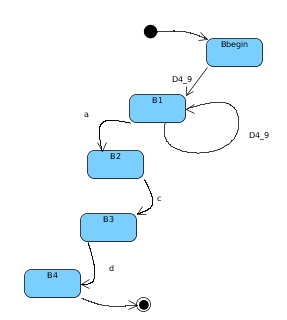
\includegraphics[scale=1]{s_b.png}
 \caption{状态机B}
 \label{fig:state_b}
\end{figure}
合并过程如下:
\begin{description}
\item[第一步:]合并状态机A与状态B的输入类型,找出相交输入类型,提取出它们的公有子集,输入类型合并的有9种:
\begin{quote}
1) 数字0到3, 命名为 D0\_3 \\
2) 数字4到7, 命名为 D4\_7 \\
3) 数字8到9, 命名为 D8\_9 \\
4) 字符a,  命名为 S\_a \\
5) 字符b,  命名为 S\_b \\
6) 字符c,  命名为 S\_c \\
7) 字符d,  命名为 S\_d \\
8) 字符f,  命名为 S\_f \\
9) 除以上字符以外的所有字符, 命名为 Other
\end{quote}
其中状态机A中的输入类型D0\_7被分解成为了输入类型D0\_3和D4\_7;状态机中的输入类型D4\_9被分解成了输入类型D4\_7和D8\_9
\item[第二步:]状态机A的开始状态为Abegin,状态机B的开始状态为Bbegin,创建一个状态复合状态 \{Abeign ,Bbegin\}, 把该复合状态命名为Cbegin,并且标记Cbegin。其中复合状态的定义为:复合状态中的任意一个状态能在某种输入类型下发生状态转移,该复合状态也能在该输入类型下发生状态转移,并且后继状态相同。
\item[第三步:]找出一个被标记的复合状态,现在只有Cbeign被标记,所以取出 Cbegin,然后取消标记 Cbeign,并确定Cbegin的后继状态,Cbeign 为 \{Abegin ,Bbegin\} 的复合状态:\\
因为:
\begin{quote}
\begin{verbatim}
f(Abegin,D0_7)->A1
f(Bbegin,D4_9)->B1
\end{verbatim}
\end{quote}
推出:
\begin{quote}
\begin{verbatim}
f(Cbegin,D0_3)->A1
f(Cbegin,D4_7)->{A1,B1}
f(Cbegin,D8_9)->B1
\end{verbatim}
\end{quote}
CBegin的转换情况如下表\footnote{空白的地方表示状态CBegin在该输入类型转移到err}:

\begin{tabular}[c]{c|c|c|c|c|c|c|c|c|c}
状态\slash输入&	D0\_3&D4\_7&D8\_9&S\_a&S\_b&S\_c&S\_d&S\_f&Other \\
\hline
CBegin&A1&A1,B1&B1&&&&&&\\
\hline
\end{tabular}

在确定后继状态,需要处理的其中的复合状态,Cbeign在输入事件D4\_7下转移到复合状\{A1,B1\},该复合状态以前并没出现过,创建复合状态\{A1,B1\},把该状态命名为C1,标记C1。
\item[第四步:] 检测现在是否存在被标记的复合状态,如果存在,跳转到第三步。如果没有,则状态机的合并完成。现在状态C1被标记,将其取出,取消标记C1,C1 为 \{A1,B1\} 的复合状态:\\
因为:
\begin{quote}
\begin{verbatim}
f(A1,D0_7)->A1
f(A1,S_a)->A2
f(B1,D4_9)->B1
f(B1,S_a)->B2
\end{verbatim}
\end{quote}
推出:
\begin{quote}
\begin{verbatim}
f(C1,D0_3)->A1
f(C1,D4_7)->{A1,B1}
f(C1,D8_9)->B1
f(C1,S_a)->{A2,B2}
\end{verbatim}
\end{quote}

C1的状态转移如下表:

\begin{tabular}[c]{c|c|c|c|c|c|c|c|c|c}
状态\slash输入&	D0\_3&D4\_7&D8\_9&S\_a&S\_b&S\_c&S\_d&S\_f&Other \\
\hline
C1&A1&A1,B1&B1&A2,B2&&&&& \\
\hline
\end{tabular}

C1的后继中状态中有两个复合状态,其中复合状态\{A1,B1\}在以前已经被创建过,所以不对其进行处理。复合状态\{A2,B2\}以前没有出现过,则创建它,并且标记,把它命名为C2。

现在还存在标记的复合状态C2,所以继续按照每二步的方法来处理,取出C2,取消标记,C2为 \{A2, B2\} 的复合状态: \\
因为:
\begin{quote}
\begin{verbatim}
f(A2,S_b)=A3
f(B2,S_c)=B3
\end{verbatim}
\end{quote}
推出:
\begin{quote}
\begin{verbatim}
f(C2,S_b)=A3
f(C2,S_c)=B3
\end{verbatim}
\end{quote}

C2的状态转移如下表:

\begin{tabular}[c]{c|c|c|c|c|c|c|c|c|c}
状态\slash输入&	D0\_3&D4\_7&D8\_9&S\_a&S\_b&S\_c&S\_d&S\_f&Other \\
\hline
C2&&&&&A3&B3&&& \\
\hline
\end{tabular}
\end{description}

现在以经没有被标记过的状态,表示状态机的整个合并过程完成,合并后创建了3个新状态:CBegin, C1, C2。每个状态接受的输入类型有9个,但可以对其进行优化,因为三个状态在输入类型 S\_d, S\_f ,Other 下都转移到err,可以把它们合并到输入类型Other中,即最终的输入类型7个:
\begin{quote}
1) 数字0到3, 命名为 D0\_3 \\
2) 数字4到7, 命名为 D4\_7 \\
3) 数字8到9, 命名为 D8\_9 \\
4) 字符a,  命名为 S\_a \\
5) 字符b,  命名为 S\_b \\
6) 字符c,  命名为 S\_c \\
7) 除以上字符以外的所有字符, 命名为 Other
\end{quote}
合并后的状态图为figure~\ref{fig:state_c}, 每个状态后继状态如下:
\begin{quote}
1) CBegin后继状态为:[A1,C1,B1,err,err,err,err]  \\
2) C1后继状态为:[A1,C1,B1,C2,err,err,err] \\
3) C2后继状态为:[err,err,err,err,A3,B3,err] 
\end{quote}
\begin{figure}
\centering
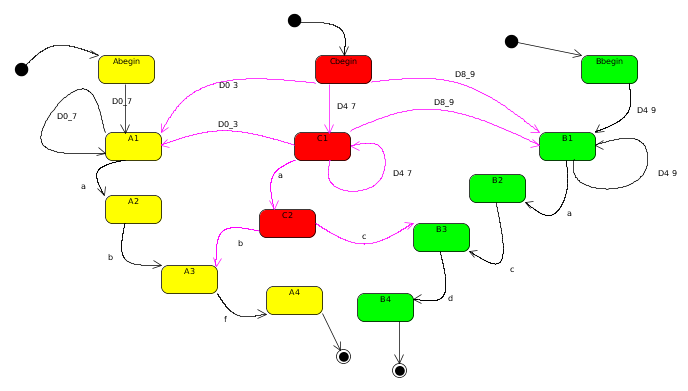
\includegraphics[scale=0.8,angle=90]{s_c.png}
\caption{状态机A与状态机B后并后}
\label{fig:state_c}
\end{figure}
状态机A与状态B的合并过程中,并不会改变状态A与状态机B的任何一个状态的信息,合并后创建了3个的新状态。新状态通过后继状态链接到子状态机A与子状态机B中的状态。把识别算法中的开始状态改为Cbegin,就可以对正则式[0-7]+abf和[4-9]+acd表示的语言进行识别。因为子状态的数据没有被改变,当只需要识别正则式[0-7]+abf所表示的语言时,同样也只需要把识别算法中的开始状态改变Abegin即可,这种特性使模块的调试变得很简单,可以先测试子状态机A和子状态机B是否正确,然后再测试合并后的状态机是否正确。

在Codger词法中有9个不同类型的单词,关键字的识别是通用先识别出标识符,然后再判断标识符是否属于关键字。子状态机有8个,识别每种单词类型子状态机的开始符号所接受的输入事件类型之间的交集很少,例如:注释以\#号开头,整数和以数字开头,浮点数以数字和点号开头,字符串以双引号开头,标识符以字母开头,在合并的时,涉及到的复合状态很少,最复杂的合并属于浮点数与整数的合并,但合并后也只创建了4个新的状态。

